\documentclass{article}
\usepackage[utf8]{inputenc}
\title{Lecture X.Y Topic}
\author{wbg231 }
\date{December 2022}
\newcommand{\R}{$\mathbb{R}$}
\newcommand{\B}{$\beta$}
\newcommand{\A}{$\alpha$}
\newcommand{\D}{\Delta}
\newcommand{\T}[1]{\Tilde{#1}}

\newcommand{\avector}[2]{(#1_2,\ldots,#1_{#2})}
\newcommand{\makedef}[2]{$\textbf{#1}$:#2 }
\usepackage{tikz,graphicx,hyperref,amsmath,amsfonts,amscd,amssymb,bm,cite,epsfig,epsf,url}

\begin{document}

\maketitle

\section{goal}
\begin{itemize}
\item correlation quantifies the dependence between two uncertain quantities with a single number 
\item we can completely characterize there dependence with a joint pmf or pdf 
\item correlation is a measure of linear dependency only (allowing us to only have a single number)
\section{linear dependence}
\item assume we have two random variables a and b, and we want to quantify the linear dependence between a and b 
\item we can do this by approximating b as a linear function of a 
\item we assume zero mean and unit variance
\item goal find best linear estimate $\beta a$ of b given a,
\item we aim to minimize the mean squared error that is $MSE(\beta)=E[(b-\beta a)^2]$ as a function of beta. this is a standard way to quantify error. we use square to avoid cancellation 
\item $MSE(\beta)=E[(b-\beta a)^2]=E[b^2=2\beta ab+\beta^2a^2]=E[b^2]+beta^2E[a^2]-2\beta E[ab]=1+\beta ^2-2\beta E[ab]$
\item now we want to optimize this as a function of beta $MSE(\beta)=1+\beta ^2-2\beta E[ab]$ then we get $MSE'(\beta)=2\beta -2E[ab]$ and $MSE''(\beta)=2$ which is convex. thus we know an extrema will be a minimum 
\item so setting $MSE'(\beta)=2\beta -2E[ab]=0$ we get $\beta_{opt} = E[ab]=\rho_{a,b}$
\item the correlation coefficient is the mean of the product between the two random variables, given a and b are standardized.
\subsection{decomposition}
\item note that b can be expressed as $b=\rho_{a,b}*a+(b-\rho_{a,b}*a)$ where $\rho_{a,b}*a$ is the best linear estimator given a and $b-\rho_{a,b}*a$ is the residual
\item note that $\rho_{a,b}\in[-1,1]$
\item if $\rho_{a,b}=0$ we say that a and b are uncorrelated
\item so the residual in this case is equal to the data. 
\item if the correlation coefficient is negative then a and b are negatively correlated.
\section{Gaussian rv}
\item what happens if a and b are both jointly Gaussian ie when they are put together they from a Gaussian random vector.
\item a Gaussian random vector has a pdf that is parameterized by a mean $\mu $ and covariance matrix $\Sigma$ 
\item with pdf 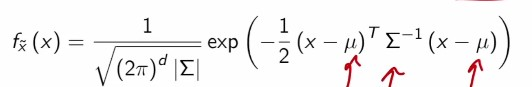
\includegraphics[width=10cm]{notes/corelation and regression/pic_1.jpg} 
\item $\mu$ tells you where the distribution is centred $\Sigma$ tells you the shape of the distribution lines of this distribution (how spread out the ellipsoid is)
\item supposed we have a Gaussian random vector (a,b) with zero mean and covariance matrix $\Sigma=\begin{pmatrix} 1 & \rho \\ \rho & 1 \end{pmatrix}$ with $\rho\in(-1,1)$
\item the entries on the main diagonal are the variance of a and b 
\item also recall because the joint Gaussian has mean zero, that both a and b has mean zero. \href{https://www.youtube.com/watch?v=adr_EwRaLbk&t=904s}{videos on Gaussian rv}
\item the parameter $\rho$ determines the covariance between a and b, $\rho\in (-1,1)$ must hold for $\Sigma$ to be positive definite and thus a valid pdf. 
\item as shown earlier the joint pdf can be expressed in terms of a marginal and conditional pdf  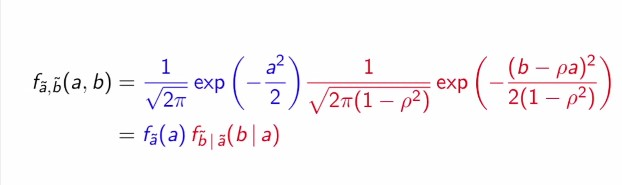
\includegraphics[width=10cm]{notes/corelation and regression/pic_2.jpg}

\item so lets study this 
\item the marginal of a is $\frac{1}{\sqrt{2\pi}}e^{-\frac{a^2}{2}}$ this is a Gaussian random variable with mean 0 and standard deviation 1 (and thus variance 1) 
\item the conditional distribution of b given a is $\frac{1}{\sqrt{2\pi(1-\rho^2)}}e^{-\frac{(b-\rho a)^2}{2(1-\rho^2)}}$ is also a Gaussian random variable with mean $\mu=\rho a $ and standard deviation equal to $\sqrt{1-\rho^2}$
\item so how does this conditional change as we vary $\rho$
\item if $\rho=0$ then $\mu=\rho *a=0, \sigma=\sqrt{1-\rho^2}=1$ meaning that the $f_{b|a}=f_{b}$ 
\item we can look at its contour lines 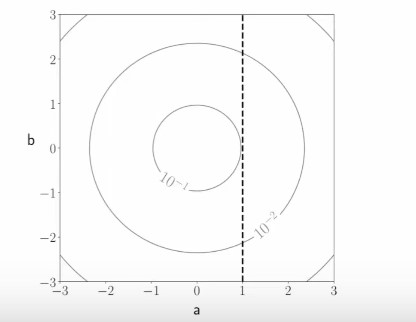
\includegraphics[width=10cm]{notes/corelation and regression/pic 3.jpg}
\item if $\rho=.05$, then $\mu=.5a, \sigma=\sqrt{1-.25}=.87$ so we have a decreased standard deviation and b is on average closer to a. 
\item we can look at its contour lines and see 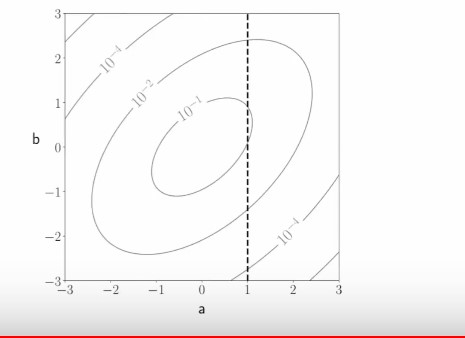
\includegraphics[width=10cm]{notes/corelation and regression/pic_4.jpg} a linear dependency start to form
\item $\rho$ determines the dependence between a and b. when $|\rho|$ is low there is no dependence. 
\item for Gaussian random variables with mean 0 and variance 1 we know that $\rho_{a,b}=E[a*b]$
\item by iterated expectations we can write $\rho_{a,b}=E[a*b]= E[\mu_{ab|a}(a)]$
\item so we know $f_{b|a}(b|a)$ has mean $\rho a$ and standard deviation $\sqrt{1-\rho^2}$
\item note that in $\mu_{ab|a}(a)$ a is fixed so we can write this as$\mu_{ab|a}(a)=\int_{a\in A}a(bf_{b|a}(b|a)db=a\mu_{b|a}(a)=a\rho a=a^2\rho$
\item so by iterated expectations and our above derivation we can see that $\rho_{a,b}=E[a*b]= E[\mu_{ab|a}(a)]=E[\rho a^2]=\rho E[a^2]=\rho$ in other words the correlation coefficient between a and b is the parameter $\rho$
\item so for Gaussian random variables there is only linear correlation determines by the correlation coefficient. 


\section{standardizing random variables}
\item to standardize a random variable $\T{a}$ we def fine a new random variable
$s(\T{a})=\frac{\T{a}-\mu_{\T{a}}}{\sigma_{\T{a}}}$
\item note that $E[S(\T(a))]=E[\frac{\T{a}-\mu_{\T{a}}}{\sigma_{\T{a}}}]=\frac{E[\T{a}]-\mu_{\T{a}}}{\sigma_{\T{a}}}=\frac{\mu_{\T{a}}-\mu_{\T{a}}}{\sigma_{\T{a}}}=0$ thus a standardized random variable has mean 0 
\item $Var(S(\T{a}))=E[s(\T{a}^2-E[s(\T{a})^2]]=E[s(\T{a}^2)]=E[\frac{(\T{a}-\mu_{\T{a}})^2}{\sigma_{\T{a}}}]=\frac{E[(\T{a}-\mu_{\T{a}})^2]}{\sigma_{\T{a}}}=\frac{\sigma}{\sigma}=1$ and thus variance equal to 1/ 
\section{linear dependence between random variables}
\item so given any two random variables $\T{a}, \T{b}$ we can standardize them and get $S(a), s(b)$
\item then we know from our above result that the best linear approximation of $s(b)$ given by $s(a)$ is $\rho_{s(a),s(b)}s(a)$
\item but notice that we can express $\T{b}$ in terms of its standardize form that is $\T{b}=\sigma_{b}s(b)+\mu_{b}$ this is just undoing the standardization
\item then as we know the best linear approximation of $s(b)$ given by $s(a)$ is $\rho_{s(a),s(b)}s(a)$ we can write $\T{b}=\sigma_{b}s(b)+\mu_{b}\approx \sigma_{b}\rho_{s(a),s(b)}s(a)+\mu_{b}=\frac{\sigma_{b}\rho_{s(a),s(b)}(a-\mu_{a})}{\sigma_{a}}+\mu_{b}$ so this is an affine approximation of b given a. 
\item so the correlation coefficient $\rho_{s(a),s(b)}$ quantifies the affine dependence between a and b 
\item so lets assert that $\rho_{s(a),s(b)}=\rho_{a,b}=E[s(a)s(b)]$
\item this works because the correlation coefficient is invariant to positive scaling and shifts due to standardization.
\item note that we can expand $E[s(a)s(b)]=E[\frac{a-\mu_{a}}{\sigma_{a}}*\frac{b-\mu_{b}}{\sigma_{b}}]=\frac{E[(a-\mu_{a})(b-\mu_{b}]}{\sigma_{a}\sigma_{b}}$
\item we define the covariance as $cov(a,b)=E[(a-\mu_{a})(b-\mu_{b}]=E[ab]-E[a]\mu_{b}-\mu_{a}E[b]+\mu_{a}\mu_{b}=E[ab]-\mu_{a}\mu_{b}-\mu_{a}\mu{b}+\mu_{a}\mu_{b}=E[ab]-\mu_{a}\mu_{b}$ 
\item note further by this definition we have $\rho_{a,b}=\frac{cov(a,b)}{\sigma_{a}\sigma{b}}$
\item this tells us that it is the affine dependence between random variables scaled to be in (-1,1)
\section{correlation and covariance}
\item if cov(a,b)$>0$ they are positively correlated 
\item if cov(a,b)=0 then they are uncorrelated. 
\subsection{example}
\item suppose we have the following joint pdf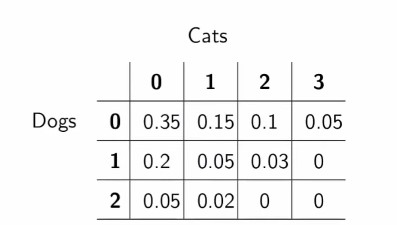
\includegraphics[width=10cm]{notes/corelation and regression/pic_5.jpg}
\item so recall that $cov(c,d)=E[c*d]-e[c]e[d]$
\item we can see that $e[c]=1*(.22)+2(.13)+3(.05)$
and $e[d]=0(.65)+1(.28)+2(.07)$
\item and $E[CD]=1*1(.05)+2(1)(.03)+2(1)(.01)=.15$
\item so finally we have $cov(c,d)=E[c*d]+e[c]e[d]=.15-(.63)(.42)=-.115$ so there is negative correlation between the number of cats and dogs. this is a simple summary of the relationship between the number of cats and dogs! 
\item then we can find the correlation coefficient as $\rho_{c,d}=\frac{COV(c,d)}{\sqrt{var(c)var(d)}}=\frac{-0.115}{(.793)(.383)}=-.208$ so when we normalize the covariance we get this correlation coefficient
\item note that this is equivalent to standardizing a and b and then finding there covariance, that is the correlation coefficient and the covariance are equal for standardized variables. 
\section{estimating covariance from data}
\item given a dataset $D=(x_1,y_1)...(x_n,y_n)$ where we have tuples of observations (we need this to understand the structure of the relationship
\item let X be the bag of the first entries, and U be the set of the second variable 
\item covariance is $cov(a,b)=E[(a-\mu_{a})(b-\mu_{b}]=E[ab]-E[a]\mu_{b}-\mu_{a}E[b]+\mu_{a}\mu_{b}=E[ab]-\mu_{a}\mu_{b}-\mu_{a}\mu{b}+\mu_{a}\mu_{b}=E[ab]-\mu_{a}\mu_{b}$
\item the sample covariance is $c(X,Y)=\frac{\Sigma_{i=1}^{n}(x-m(X))(y-m(Y))}{n-1}$
\item where m(X) is the sample mean of X 
\item we divide by n-1 to make sure it is unbiased (often does not mater much in practice) 
\item the sample correlation coefficient is $\rho_{X,Y}=\frac{c(X,y)}{\sqrt{V(X)V(Y)}}$ where $V(X)$ is the sample variance of X
\item so sample correlation coefficient is a scaled version of sample covariance
\item the correlation coefficient is the optimal linear scaling between random variables 
 \subsection{standardized data}
 \item given dataset X=$\{x_1,...x_n\}$
 we can define $s(x_i)=\frac{x_i-m(X)}{\sqrt{v(X)}}$ 
 \item this allow us to write given a dataset with tuples (x,y) $\rho_{x,y}=\frac{1}{n-1}\Sigma_{i=1}^{n}\frac{(x_i-m(X))(y_i-m(Y))}{\sqrt{V(x)V(y)}}=\frac{1}{n-1}\Sigma_{i=1}^{n}\frac{(x_i-m(X))}{\sqrt{V(x)}}\frac{(y_i-m(Y))}{\sqrt{V(y)}}=\frac{1}{n-1}\Sigma_{i=1}^{n}s(x_i)s(y_i)$ so this is something equivalent to the mean of the product of the standardized variables. 
 \item recall that for standardized data the sample mean is 0 and the sample variance is 1, so  the sample variance is equal to the sample mean squared. $v(s(x))=m(s(x)^2-m(s)^2)=m(s(x)^2)=1=\frac{1}{n-1}\Sigma_{i=1}^{n}s(x_i)^2$ and thus $n-1=\Sigma_{i=1}^{n}s(x_i)^2$
 \section{residual sum of squares}
 \item given a data set $D=(x_1,y_1)...(x_n,y_n)$
 \item how can we approximate $s(y_i)$ by scaling $s(x_i)$?
\item we cant do means because we are dealing with data but we can use the residual sum of squares $RSS(\beta)=\Sigma_{i=1}^{n}(s(y_i)-\beta s(x_i))^2$ so we are averaging the sum of squared error between what we are trying to estimate and our approximate 
\item we can expand this sum as $RSS(\beta)=\Sigma_{i=1}^{n}(s(y_i)-\beta s(x_i))^2=\Sigma_{i=1}^{n}s(y_i)^2+\beta^2\Sigma_{i=1}^{n}s(x_i)^2-2\beta \Sigma_{i=1}^{n} s(x_i)s(y_i)=(n-1)+\beta^2(n-1)-2\beta \Sigma_{i=1}^{n} s(x_i)s(y_i)=(n-1)+\beta^2(n-1)-2\beta (n-1) \rho_{x,y}=(n-1)(1+\beta^2-2\beta \rho_{x,y}$
\item taking the derivative with respect to beta we get $rss(\beta)'=2\beta(n-1) -2\rho_{x,y}(n-1)$
\item taking the second derived we get $rss(\beta)''=2(n-1)>0$ so it is convex 
\item thus if the first derivative is equal to zero we will have a global min ie  $rss(\beta)'=2\beta(n-1) -2\rho_{x,y}(n-1)=0$ meaning $\beta_{ols}=\rho_{x,y}$
\item so in other words the optimal way to estimate the standardized second variable by the first variable in a linear way we would use the correlation coefficient
\section{simple linear regression}
\item we have a single feature that we are going to use to construct an affine estimator of outcome variable written as $b\approx\beta a+\alpha$
\item so we are modeling b as a scaled version of a plus some constant 
\item in a previous video we showed that the best linear approximation of a standardized random variable s(b) given another standard variable s(a) is s(a) scaled by there co relation coefficient that is $\rho_{s(a),s(b)}s(a)$
\item we can then general this to any random variables a and b as $b=\sigma_{b}s(b)+\mu_{b}\approx \sigma_{b} \rho_{s(a),s(b)}s(a)+\mu_{b}=\frac{\sigma_{b}\rho_{s(a),s(b)}(a-\mu_{a}}{\sigma_{a}}+\mu_{b}$ 
\item so this allows us to express the best linear approximation of b as an affine function of a
\subsection{linear MMSE Estimator}
\item suppose we want to find the best parameters $\beta, \alpha$ such that $\beta, \alpha=argmin_{\alpha,\beta}E[(b-\beta a-\alpha)^2]$
\item keep in mind that the best constant estimator of a random variable x is the $E[x]$ that is $argmin_{c\in \mathbb{R}}E[(c-x)^2]=E[x]$ 
\item so if we think of $b-\beta a$ as a random variable then the constant $\alpha$ which minimizes it best is $\alpha_{mmse}(b)=E[b-\beta a]=E[b]-\beta E[a]=\mu_{b}-\beta \mu_{a}$
\item so that is the best alpha for any given value of beta, thus we can think of alpha as a function beta and reduce the problem to 1 variable, that is $\beta_{mmse}=argmin_{\beta}MSE(\beta,\alpha*(\beta))$ 
\item $MSE(\beta,\alpha*(\beta))=E[(b-\beta a -\alpha^{*}(\beta))^2]=E[(b-\beta a -\mu_{a}+\beta \mu_{a})^2]=E[(b-\mu_{b})^2]+\beta^2E[(a-\mu_{a})^2]-2\betaE[(a-\mu_{a})(b-\mu_{b})]=\sigma_{a}+sigma_{b}-2cov[a,b]\beta$
\item so now we can minimize this $MSE(\beta)'=2\beta \sigma_{a}-2cov[a,b]$ and the second derivative is $2\sigma_{a}^2$ so the function is convex, this means we have a global minima at $MSE(\betae)'=2\beta \sigma_{a}-2cov[a,b]=0$ yielding $\beta_{mse}=\frac{cov(a,b)}{\sigma_{a}}$
\item recall that $cov(a,b)=\rho_{a,b}\sigma_{b}$ so we can write $\frac{cov(a,b)}{\sigma_{a}}=\frac{\rho_{a,b}\sigma_{b}}{\sigma_{a}}$
\item so call the optimal linear estimator in terms of Mean squared error $l(a)$ and note that we can write $l(a)=\beta_{mmse}a+\alpha_{mmse}=\beta_{mmse}a+\mu_{b}-\beta\mu_{a}=\beta(a-\mu_{a})+\mu_{b}=\rho_{a,b}\sigma_{b}\frac{a-\mu_{a}}{\sigma_{a}}+\mu_{b}$
\item this is the same as what we got with our argument about correlation so that is good. 
\subsection{example}
\item suppose we have the following joint pdf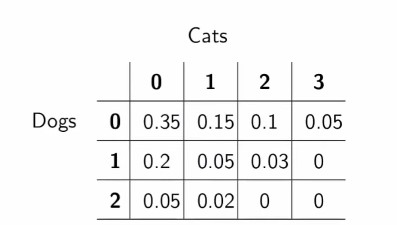
\includegraphics[width=10cm]{notes/corelation and regression/pic_5.jpg}
\item we can compute the optimal linear estimator of c given d as $l(d)=\sigma_c\rho_{c,d}\frac{d-E{d}}{\sqrt{var(d)}}+E{c}=-.3d+.756$
\item this is the best linear estimate of the number of cats given the number of dogs. this is consistent with what we saw in the last example as the correlation between cats and dogs are negative 
\item the mean squared error of this is $E[(c-l(d))^2]=\Sigma_{d=1}^{2}\Sigma_{c=1}^{3}P_{c,d}(c+.3d-.756)^2=0.759$
\item is this estimator optimal? no the conditional mean will reduce in a lower mean squared error estimator. using the the conditional mean to estimate the same problem yields a mean squared error of .76 which is pretty close to that of the linear estimator. meaning there is a strong linear relationship in the data. 
\item but the linear estimator is constrained to lie on a line! where as the conditional mean can be any function it can depart from a line as much as it wants. 
\item so in general using a non-linear estimator will yield more flexibility, but may not necessarily improve mse that much, further it may capture more sub groups in the data that may not be caught with a line just fit to the data with one variable.
\item while the linear estimator just relies on the correlation coefficient and is Nice and simple, further it will preform better on low amounts of data. .
\section{Gaussian random variables}
\item assume that the feature and response a and b are jointly Gaussian forming the Gaussian random vector \begin{pmatrix}a\\b\end{pmatrix} with mean \begin{pmatrix}\mu_{a}\\\mu_{b}\end{pmatrix} with covariance $\Sigma=\begin{pmatrix}
    \sigma_{a}^2 & \rho\sigma_{a}\sigma_{b}\\\rho\sigma_{a}\sigma_{b} & \sigma_{b}^2
\end{pmatrix}$
\item what is the minimum MSE estimator of b given a? the conditional mean function
\item however recall that the conditional mean function for Gaussian random vectors of this type is the same as the best linear estimator $\mu_{b|a}(a)=\frac{\rho \sigma_{b}(a-\mu_{a})}{\sigma_{a}}+\mu_{b}$
\item so this shows that the dependence between Gaussian rv's is completely linear 
\subsection{simple linear regression }
\item given dataset $(x_1,y_1)...(x_n,y_n)$
\item how do we construct a linear estimate? 
\item we can think of x as coming form an rv a and y as coming from an rv b.
\item we showed earlier that for random variables we can get the best minima mse linear estimator as $l(a)=\sigma_{b}\rho_{a,b}\frac{a-\mu_{a}}{\sigma_{b}}+\mu_b$ so we can approximate this with the sample estimates 
\item that is $l(a)=\sigma_{b}\rho_{a,b}\frac{a-\mu_{a}}{\sigma_{b}}+\mu_b\approx\sqrt{v(X)}\rho_{X,y}(\frac{x-M(x)}{\sqrt{V(x)}})+M(y)$ 
\item we can also minimize the sum of squared error over the data, and use sample average and we get the same outcome for an minimum mean squared error estimator. 
\end{itemize}
\end{document}
